\documentclass[11pt]{article}
\usepackage[margin=1in]{geometry}
\usepackage[T1]{fontenc}
\usepackage{lmodern}
\usepackage{microtype}
\usepackage{amsmath,amssymb}
\usepackage{booktabs}
\usepackage{graphicx}
\usepackage{xcolor}
\usepackage[numbers,sort&compress]{natbib}
\usepackage[colorlinks=true,linkcolor=blue!50!black,citecolor=blue!50!black,urlcolor=blue!50!black]{hyperref}

\newcommand{\ci}[2]{\,[#1,\,#2]}

\title{Topic Momentum Forecasts Which Astronomy Questions the Field Takes Up:\\
Five Pre-registered Out-of-Time Backtests and a Sealed 2026--2031 Forecast}
\author{Hui Mao\\ Aurora AI Ventures \and Claude Code\\ Anthropic}
\date{October 2026}

\begin{document}
\maketitle

\begin{abstract}
Can we tell, from the literature available on a given day, which research
questions a field will substantively take up over the following years? Earlier
work in this series built an evidence-graph question generator, a historical
backtesting protocol, and a predictor of future attention fitted on 980
astronomy questions at cutoffs 2012--2020. Here we test that predictor, and two
successors, where it matters: at cutoffs none of them has seen. We ran four
pre-registered rounds, each committed publicly before its questions existed.
Every prediction was frozen with SHA-256 digests and pushed before any outcome
was labelled. The test material is 995 questions at five new cutoffs (2017,
2019, 2021, 2022, 2023) across eight astronomy subfields, scored against a
332,244-paper arXiv astro-ph corpus, with outcome windows running to October
2026. The original predictor transfers forward in time (AUC 0.63--0.69 at every
cutoff) but does no better than knowing how a question was generated. Adding
the question's embedding and \emph{topic momentum}, meaning how many and how
recent the pre-cutoff papers near the question are, yields a model (v3) that
reaches AUC 0.769 on the fresh 2017 and 2023 cohorts. It beats the
generation-source prior by $+0.081\ci{0.042}{0.123}$, ranks questions within a
source at 0.694, and is the best-calibrated model (Brier 0.191). We then test
the three main threats to such results. Against a citation-graph outcome label
that uses no text retrieval, v3 keeps AUC 0.680 (momentum alone 0.689). On 595
questions written with no language model, it scores 0.693; LLM phrasing
inflates outcome rates by 16 points but not the ranking. On 90 questions
labelled independently by two humans, it predicts their judgments (AUC
0.66--0.70) better than it predicts the LLM judge. The same human data shows
that the strict LLM judge underlying every label in this line of work is far
more conservative than human readers ($\kappa\approx0$--$0.14$), whose own
agreement is only $\kappa=0.11$. A planning component from the series (Paper~4)
has no predictive value. Finally, we seal a v3 forecast for 200 questions posed
on 2026-10-14, to be scored after 2031-10-15. All code, data, caches, and the
commit history that timestamps each step are public.
\end{abstract}

\section{Introduction}

Systems that propose scientific questions are usually judged by how good the
questions look to a person or a model. A more demanding standard asks whether
the field actually went where the questions point. Historical backtesting turns
that standard into a measurement~\cite{mao2026backtesting}:
\begin{itemize}
\item generate questions from literature published before a cutoff;
\item freeze them;
\item label each one by what the following years of literature did with it.
\end{itemize}
The third paper in this series used the protocol to fit a predictor of future
attention on 980 astronomy questions at cutoffs 2012--2020. It reported a
temporal-split AUC of 0.71.

A predictor tuned on a fixed set of cutoffs can look good for reasons that do
not survive time. This paper asks whether the forecast holds up when it is made
the way a forecaster would actually have made it: at a cutoff the model never
saw, trained only on outcomes that were already known on that day, and scored
before anyone looks at the answers.

\paragraph{Contributions.}
\begin{enumerate}
\item \textbf{Out-of-time replication.} Paper~3's predictor transfers to five
  new cutoffs (pooled AUC 0.655 over 995 questions). Most of that skill,
  however, is a generation-source prior (\S\ref{sec:r1}).
\item \textbf{Topic momentum.} A dense-retrieval measure of how much, and how
  recently, the field was already publishing near a question is the strongest
  single predictor we found. Combined with the question's embedding (v3), it
  reaches AUC 0.77 and within-source AUC 0.69 on fresh cutoffs, under
  pre-registered tests (\S\ref{sec:r3}).
\item \textbf{Three validity checks.} We test the forecast against a
  citation-graph outcome that bypasses text retrieval, against questions
  written with no language model, and against human judgments
  (\S\ref{sec:validity}). It survives all three.
\item \textbf{A measurement finding.} The strict LLM judge behind the series'
  labels is far stricter than humans, and humans barely agree with each other.
  Absolute outcome rates are therefore rater-relative, and LLM-phrased
  questions inflate them further (\S\ref{sec:judge}).
\item \textbf{A sealed forecast.} 200 questions posed on 2026-10-14 are
  scored by three model versions, frozen, and due for scoring after 2031-10-15
  (\S\ref{sec:prospective}).
\end{enumerate}

\section{Related work}

\paragraph{Forecasting the direction of science.} Embeddings trained on past
literature can anticipate future findings: word embeddings of materials-science
abstracts ranked compounds that were later reported for a property years before
publication~\cite{tshitoyan2019}. Semantic networks built from past papers
predict which concept pairs will be studied together in quantum
physics~\cite{krenn2020} and in AI~\cite{krenn2023}. Human-aware models that
account for who can make a connection forecast discoveries better than
content-only models~\cite{sourati2023}. Our task differs from all of these in
three ways:
\begin{itemize}
\item the unit is a natural-language \emph{research question}, not a concept
  pair or material;
\item the outcome is \emph{substantive engagement}, judged from later papers;
\item every evaluation is pre-registered and out of time.
\end{itemize}

\paragraph{Predictability in the science of science.} The science of science
has long studied what can and cannot be predicted about papers and
careers~\cite{clauset2017}, for example long-term citation
impact~\cite{wang2013}. We predict uptake of \emph{questions}, a step earlier
than impact. Our momentum features are close in spirit to field-growth
predictors, but they are measured per question.

\paragraph{LLM-generated ideas and LLM judges.} Expert evaluation finds
LLM-generated research ideas judged more novel but less feasible than human
ones~\cite{si2024}. Our backtests replace expert opinion with observed outcomes,
but they rely on an LLM judge. Known judge biases~\cite{zheng2023} and our own
human comparison (\S\ref{sec:judge}) make that judge a measured instrument
rather than ground truth.

\paragraph{This series.} Paper~1~\cite{mao2026framework} generates questions
from tensions in an evidence graph. Paper~2~\cite{mao2026backtesting}
formalises historical backtesting and includes a blinded two-annotator study
that we reuse. Paper~3 (pending) provides the 980-question training set, the
six feature groups, the label pipeline and the v1 model. Paper~4 (pending)
ranks next evidence-gathering actions for a question. All upstream code and
data are vendored unmodified at pinned commits.

\paragraph{Pre-registration.} Freezing hypotheses and analysis plans before
seeing outcomes~\cite{nosek2018} is the main defence against tuning to the test
set. We apply it to forecasting: the forecast itself is frozen and its digest
published before the outcomes are computed.

\section{Setup}\label{sec:setup}

\paragraph{Corpus.} We harvested arXiv astro-ph metadata, including
cross-lists, from 2005 to 2026-10-14 through OAI-PMH: 332,244 papers. The
publication date is the version-1 date. The per-year counts match Paper~3's
independent harvest: identical for 2007--2021 and within 0.06\% elsewhere.
Paper~3's keyword rules assign papers to eight subfields:
\begin{itemize}
\item exoplanet atmospheres;
\item protoplanetary disks;
\item stellar activity;
\item fast radio bursts;
\item gravitational waves;
\item galaxy evolution;
\item cosmology tensions;
\item compact objects.
\end{itemize}
The 106,428 subfield papers are embedded with \texttt{text-embedding-3-small}.

\paragraph{Questions.} For every cutoff and subfield, Paper~3's generators
produce 25 questions from the preceding eight years of abstracts only:
\begin{itemize}
\item 10 \emph{evidence-tension} questions, from clusters of contradiction
  statements across at least two papers (Paper~1's approach);
\item 5 \emph{direct-LLM} questions;
\item 5 \emph{author future-work} questions;
\item 5 weak or negative \emph{controls}.
\end{itemize}
Phrasing uses \texttt{gpt-4o-mini}. The five test cutoffs yield 995 questions;
one small 2017 cell produced only 5 tension clusters.

\paragraph{Outcome label.} A question is \emph{addressed} if, among the top-8
post-cutoff papers of its subfield retrieved by TF-IDF, Paper~3's strict judge
(\texttt{gpt-4o}) finds at least one that engages it directly and assigns an
outcome other than \texttt{not\_addressed}.

The outcome windows are:
\begin{itemize}
\item five years for the 2017 and 2019 cutoffs;
\item to 2026-10-14 for the later cutoffs: 4.79, 3.79 and 2.79 years for 2021,
  2022 and 2023.
\end{itemize}
Base rates range from 0.495 to 0.605.

\paragraph{Leak-free training.} Each test cohort is scored by models fitted
only on Paper~3 questions whose outcome windows had \emph{closed} by the test
cutoff:
\begin{center}
\begin{tabular}{@{}ll@{}}
\toprule
Test cutoff & Training cutoffs \\
\midrule
2017 & 2012 \\
2019 & 2012, 2014 \\
2021, 2022 & 2012, 2014, 2016 \\
2023 & 2012, 2014, 2016, 2018 \\
\bottomrule
\end{tabular}
\end{center}
A model trained on later labels would see field dynamics from inside the test
window.

\paragraph{Pre-registration and freezing.} Each round's hypotheses, metrics and
decision rules were committed to the public repository before that round's
questions were generated. Questions, features and predictions were then frozen
with SHA-256 digests and pushed before labelling. Models were designed only on
cohorts whose labels had already been seen:
\begin{itemize}
\item v2 on the 2021 cohort;
\item v3 on 2019, 2021 and 2022, plus leave-one-cutoff-out on Paper~3.
\end{itemize}
Confirmatory claims use only cohorts generated afterwards. Bootstrap intervals
use 2,000 resamples stratified by cohort $\times$ source.
\emph{Within-source AUC} is the mean AUC over cohort $\times$ source strata
that contain both outcome classes.

\section{Models}\label{sec:models}

\paragraph{v1: Paper~3's model.} This is a logistic regression on six groups of
cutoff-time features: text, evidence context, novelty, falsifiability,
tractability and field environment. Our vendored copy reproduces Paper~3's
published temporal-split AUC exactly (0.7126).

\paragraph{v2: embedding with a source fixed effect.} This is a logistic
regression on the question's embedding plus one-hot generation source. The
fixed effect forces the remaining features to explain variation \emph{within}
a source. C is chosen by leave-one-cutoff-out AUC on the training set. A
calibrated variant averages its log-odds with v1's features (plus the source
effect) and applies Platt scaling on out-of-fold predictions.

\paragraph{v3: adding topic momentum.} For each question we compute cosine
similarities between its embedding and every paper of its subfield in the
eight-year past window, and derive nine features:
\begin{itemize}
\item mean similarity of the 10 and the 50 nearest papers;
\item log-counts of papers above two similarity thresholds (0.58 and 0.65,
  set from the feature distribution, not from outcomes);
\item that count as a share of the subfield;
\item the share of the 50 nearest papers from the last two years;
\item the mean age of the 20 nearest papers;
\item the log-ratio of near papers in the last two years to the two years
  before;
\item the count of near papers in the last two years.
\end{itemize}
v3 averages the log-odds of a momentum-plus-source logistic model and v2's
embedding model, with the same Platt calibration. Its training cohorts never
include the test cutoff.

\section{Results}\label{sec:results}

\subsection{The original predictor transfers, but mostly as a source prior}\label{sec:r1}

At cutoff 2021, the first round, v1 scored AUC 0.656\ci{0.583}{0.733},
against 0.71 within its own era:
\begin{itemize}
\item it beat a subfield-popularity baseline by $+0.102\ci{0.039}{0.167}$;
\item it did \emph{not} beat a one-number-per-source prior
  ($-0.024\ci{-0.109}{0.073}$);
\item its within-source AUC was 0.569\ci{0.496}{0.650}.
\end{itemize}
Across all five cutoffs v1 is stable (Table~\ref{tab:cutoffs}): pooled AUC
0.630--0.693. Its ranking of direct-LLM questions is at or below chance
(pooled 0.44), because those questions are engaged almost regardless of
content.

\begin{table}[t]
\centering
\caption{AUC by cutoff, as pooled / within-source, under Paper~3's label. Each
cohort is scored by models trained only on labels closed by its cutoff.
\emph{dev} marks cohorts a model was designed on. Bold marks fresh tests of v3.}
\label{tab:cutoffs}
\small
\begin{tabular}{@{}lcccc@{}}
\toprule
Cutoff ($n$) & v1 (Paper~3) & source prior & v2 & v3 \\
\midrule
2017 (195) & 0.630 / 0.577 & 0.628 / 0.50 & 0.674 / 0.594 & \textbf{0.728 / 0.634} \\
2019 (200) & 0.654 / 0.548 & 0.667 / 0.50 & 0.730 / 0.642 & 0.765 / 0.703 \emph{(dev)} \\
2021 (200) & 0.656 / 0.569 & 0.680 / 0.50 & 0.745 / 0.646 \emph{(dev)} & 0.784 / 0.704 \emph{(dev)} \\
2022 (200) & 0.677 / 0.648 & 0.667 / 0.50 & 0.747 / 0.650 & 0.776 / 0.687 \emph{(dev)} \\
2023 (200) & 0.693 / 0.609 & 0.758 / 0.50 & 0.827 / 0.738 & \textbf{0.845 / 0.753} \\
\midrule
All (995) & 0.655 / 0.590 & 0.686 / 0.500 & 0.738 / 0.654 & 0.771 / 0.696 \\
\bottomrule
\end{tabular}
\end{table}

\subsection{An embedding model beats the source prior}\label{sec:r2}

On the fresh 2019 and 2022 cohorts ($n=400$), v2 was tested against
pre-registered hypotheses:
\begin{itemize}
\item pooled AUC 0.737 against the source prior's 0.669, a gain of
  $+0.068\ci{0.019}{0.117}$;
\item within-source AUC 0.646\ci{0.583}{0.710};
\item AUC 0.606\ci{0.515}{0.694} within evidence-tension questions;
\item Brier score 0.207, against v1's 0.240 and the constant's 0.248.
\end{itemize}
Its within-source gain over v1 (+0.048) was not significant. v1 also scored
above chance within sources on these cohorts (0.598), so part of round~1's
within-source failure was specific to the 2021 cohort.

\subsection{Topic momentum: the strongest predictor}\label{sec:r3}

Table~\ref{tab:r3} reports the round-3 tests on the fresh 2017 and 2023
cohorts ($n=395$, base rate 0.51). v3:
\begin{itemize}
\item ranks within a source at 0.694 (T1);
\item beats v1 within a source by $+0.101$ (T3);
\item beats the source prior by $+0.081$ (T4);
\item ranks evidence-tension questions at 0.692 (T6);
\item has the best Brier score (T5).
\end{itemize}
Its within-source gain over v2, $+0.028\ci{-0.008}{0.062}$, misses
significance (T2). Across all five cutoffs v3 is the best model on both
measures in every cohort (Table~\ref{tab:cutoffs}). The momentum model alone
reaches pooled AUC 0.770 on the fresh cohorts. Its strongest contribution is
inside evidence-tension questions: 0.738, against 0.599 for v2.

\begin{table}[t]
\centering
\caption{Round 3: pre-registered tests on the fresh 2017 and 2023 cohorts.}
\label{tab:r3}
\small
\begin{tabular}{@{}llc@{}}
\toprule
ID & Hypothesis & Result \\
\midrule
T1 & v3 ranks within a source & AUC 0.694\ci{0.612}{0.771} \checkmark \\
T2 & v3 $>$ v2 within a source & $\Delta=+0.028\ci{-0.008}{0.062}$, not significant \\
T3 & v3 $>$ v1 within a source & $\Delta=+0.101\ci{0.027}{0.176}$ \checkmark \\
T4 & v3 $>$ source prior (pooled) & 0.769 vs 0.688; $\Delta=+0.081\ci{0.042}{0.123}$ \checkmark \\
T5 & Brier(v3) $<$ Brier(v2) & 0.191 vs 0.206 (v1 0.253) \checkmark \\
T6 & v3 ranks evidence-tension questions & AUC 0.692\ci{0.604}{0.773} \checkmark \\
\bottomrule
\end{tabular}
\end{table}

\begin{figure}[t]
\centering
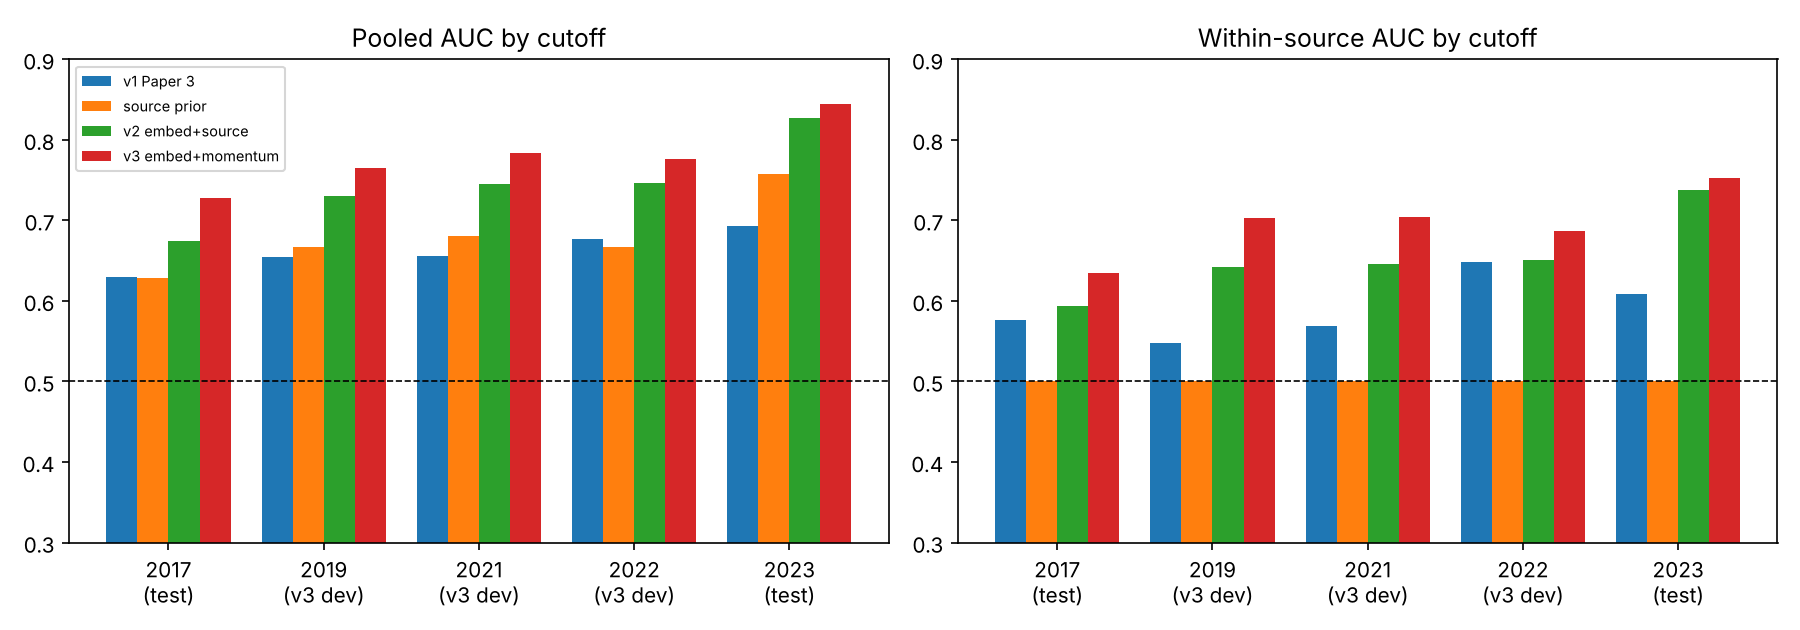
\includegraphics[width=\linewidth]{figures/auc_by_cutoff.png}
\caption{Pooled (left) and within-source (right) AUC at each cutoff. Cohorts
marked \emph{dev} were used to design v3; 2017 and 2023 are fresh tests.}
\label{fig:cutoffs}
\end{figure}

\section{Validity checks}\label{sec:validity}

Figure~\ref{fig:forest} summarises v3's skill under every check in this
section.

\begin{figure}[t]
\centering
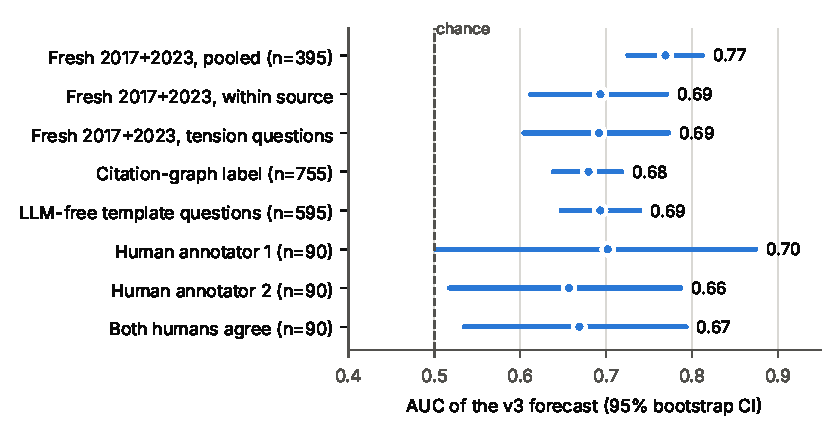
\includegraphics[width=0.85\linewidth]{figures/forest_v3.pdf}
\caption{v3's AUC, with 95\% bootstrap intervals, on the fresh test cohorts and
under the three validity checks: a retrieval-independent citation label,
LLM-free questions, and human annotators.}
\label{fig:forest}
\end{figure}

\subsection{Is momentum just predicting the retriever?}
The outcome label finds future papers by TF-IDF similarity, and momentum counts
past papers similar to the question. Momentum could therefore predict the
retriever instead of the field.

We built a second label whose candidates are post-cutoff papers that
\emph{cite the question's source papers}, taken from the Semantic Scholar
citation graph (1,213 of 1,214 source papers). It is judged by the same
\texttt{gpt-4o} rubric. It is defined for the 755 questions that have source
papers, across all five cutoffs, and agrees with the TF-IDF label on 73\% of
them.

On this label:
\begin{itemize}
\item v3 scores AUC 0.680\ci{0.639}{0.718};
\item the momentum model alone scores 0.689\ci{0.650}{0.730}, almost unchanged
  from its 0.699 on the TF-IDF label;
\item v1 falls from 0.614 to 0.569.
\end{itemize}
Momentum tracks where the field went, not how the retriever works.

\subsection{Did the question generator leak the future?}
The generator (\texttt{gpt-4o-mini}) has read literature from after every
backtest cutoff. To test whether that matters, we pre-registered and built 595
questions with \emph{no language model}: the same tension clusters and
future-work sentences, inserted verbatim into fixed templates. Each of the 395
tension templates shares its evidence cluster with exactly one LLM-phrased
question.

\begin{itemize}
\item \textbf{v3's skill holds.} It scores 0.693\ci{0.648}{0.739} pooled and
  0.704\ci{0.657}{0.750} within template type.
\item \textbf{LLM phrasing inflates outcome rates.} On the same 395 clusters,
  the LLM-phrased question is addressed 44.6\% of the time and the template
  28.6\%: $+16.0$ points\ci{10.9}{21.0}.
\item \textbf{The ranking does not depend on phrasing.} v3's AUC is 0.726 on
  the templates against 0.679 on their LLM-phrased twins
  ($\Delta=+0.047\ci{-0.032}{0.121}$).
\end{itemize}
Absolute outcome rates of LLM-generated questions should therefore not be
quoted as properties of the questions. Rankings are unaffected.

\subsection{Do the forecasts predict human judgment?}\label{sec:judge}
Paper~2's blinded study had two annotators label 90 questions (cutoff 2020),
each shown the same eight post-cutoff abstracts a judge sees. We ran Paper~3's
judge on those items.

The judge and the humans disagree:
\begin{itemize}
\item humans call 90\% and 73\% of the questions addressed;
\item the strict \texttt{gpt-4o} judge calls 43\% addressed;
\item agreement with each human is $\kappa=-0.00$ and $0.14$;
\item the two humans agree with each other at only
  $\kappa=0.11\ci{-0.08}{0.32}$.
\end{itemize}

We also checked that the judge itself is stable. Re-judging 120 of Paper~3's
own questions today, \texttt{gpt-4o} reproduces the committed labels
($\kappa=0.83$, identical 50.8\% rate). \texttt{gpt-4o-mini}, the pipeline's
code default, calls 93\% addressed ($\kappa=0.14$).

Scored with v3 trained only on cutoffs that closed by 2020, the 90 questions'
forecasts predict:
\begin{itemize}
\item human~1, AUC 0.702\ci{0.502}{0.874};
\item human~2, 0.657\ci{0.518}{0.787};
\item questions both humans call addressed, 0.669\ci{0.535}{0.793};
\item the \texttt{gpt-4o} judge on the same items, only 0.548.
\end{itemize}
The forecast signal therefore reaches human judgment and is not an artefact of
the judge's rubric. This analysis was not pre-registered, and $n=90$ is small.

\subsection{Negative result: the evidence planner}
Paper~4's planner ranks next evidence-gathering actions. Its top-$k$ utility
does not predict uptake: AUC 0.419\ci{0.305}{0.537} within tension questions
at cutoff 2021, replicating Paper~4's own retraction.

Its top-ranked action is nearly constant. Under the default configuration it
recommends a simulation for 41 of the 42 questions that were followed up.
Under the Paper-3-informed configuration it recommends a literature review for
all of them. It matches the action the field actually took (classified by
\texttt{gpt-4o}) at 0.60, against a permutation null of 0.61 ($p=1.0$).

\section{A sealed 2026--2031 forecast}\label{sec:prospective}

On 2026-10-14 we generated 200 new questions with the same generators and
scored them with v1, v2 and v3. Each version's scores are frozen separately
(\texttt{FREEZE*.json}). They will be labelled with the same pipeline over
2026-10-15 to 2031-10-14, no earlier than 2031-10-15. The pre-registered claims
are:
\begin{itemize}
\item AUC $>0.5$;
\item the top quintile is addressed more often than the bottom quintile.
\end{itemize}
Paper~2's 200 questions, frozen on 2026-08-17, are scored the same way.

The forecast is about \emph{uptake}, not answers. A score of 0.75 means the
model expects at least one post-cutoff paper to engage the question directly
and substantively, with new evidence, a test or a resolution attempt. It makes
no claim about \emph{what} that work will find, or whether the question will be
settled. Resolutions are too rare in the historical labels (8 of Paper~3's
980 questions) for that to be forecastable at this scale.

v3's mean forecast is highest for fast radio bursts (0.62) and cosmology
tensions (0.60), and lowest for stellar activity (0.42). Among the
evidence-tension questions, the top-ranked concern:
\begin{itemize}
\item the Hubble-constant discrepancy and early-dark-energy resolutions
  (0.65--0.75);
\item the abundance of luminous $z>10$ galaxies seen by JWST (0.70--0.75);
\item magnetar and merger-remnant origins of fast radio bursts (0.65--0.73);
\item the $\sim$2.5\,$M_\odot$ object in GW190814 and the black-hole mass gap
  (0.66--0.67).
\end{itemize}
The lowest-ranked are narrow object-level discrepancies (0.19--0.28), such as
retrieved C/O ratios of Gliese~229\,B or spot coverage of HAT-P-12.

\section{Limitations and deviations}

\begin{itemize}
\item \textbf{The label is an instrument, not ground truth.} ``Addressed''
  means addressed according to a strict \texttt{gpt-4o} rubric over
  abstract-level retrieval. Human annotators are both more lenient and
  mutually inconsistent. Our human check ($n=90$) supports the forecast's
  validity but is underpowered.
\item \textbf{Shorter windows at recent cutoffs.} The 2021--2023 cohorts have
  outcome windows of 2.8--4.8 years, against five years for Paper~3.
\item \textbf{One domain, one corpus.} Astronomy only, arXiv only, eight
  keyword-defined subfields.
\item \textbf{Generator leakage.} It affects outcome rates (+16 points) but
  not the ranking. Remaining embedding-model leakage was not tested separately.
\item \textbf{Deviations from pre-registration, all disclosed in the
  repository.}
  \begin{itemize}
  \item Round~1 named the wrong judge model: the code default
    \texttt{gpt-4o-mini} instead of \texttt{gpt-4o}, which made Paper~3's
    labels. We report both and use the latter.
  \item The citation label was delayed by API rate limits, and its round-1
    analyses are exploratory.
  \item v2 received the single-training-cutoff rule pre-stated for v3, to be
    scorable at 2017. This leaves multi-cutoff predictions byte-identical.
  \end{itemize}
\item \textbf{T2 failed.} v3's within-source improvement over v2 is not
  significant. Its advantage is significant against v1 and the source prior.
\end{itemize}

\section{Conclusion}

Across five pre-registered out-of-time cutoffs, a forecaster built from this
series' components predicts which astronomy questions the field will take up.
The decisive ingredient is not the structure of the question but \emph{topic
momentum}: whether the field was already moving toward it at the cutoff.

The forecast survives three checks:
\begin{itemize}
\item an outcome label that bypasses text retrieval;
\item questions no language model wrote;
\item human judgment.
\end{itemize}
The work also measures, rather than assumes, how much its LLM instruments
shape absolute rates.

The sealed 2026--2031 forecast is the test no backtest can replace. Every
model that exists today will be scored on literature none of them has seen.

\paragraph{Data and code.}\leavevmode\\
\url{https://github.com/nonameisready/scientific-discovery-astronomy}.
This contains:
\begin{itemize}
\item pre-registrations \texttt{docs/PREREGISTRATION*.md};
\item frozen predictions and digests (\texttt{data/*/FREEZE*.json});
\item labels and LLM caches;
\item scripts reproducing every number in this paper.
\end{itemize}

\bibliographystyle{plainnat}
\bibliography{references}

\appendix
\section{Timeline of commits}\label{app:timeline}
Each step below is a public commit, so the order is verifiable.

\begin{center}
\small
\begin{tabular}{@{}ll@{}}
\toprule
Commit & Step \\
\midrule
\texttt{bcf8469} & Round-1 pre-registration (cutoff 2021), before any question \\
\texttt{60f0f5d} & 2021 cohort and predictions frozen, before any label \\
\texttt{a4eea0f} & Round-2 pre-registration and v2 models \\
\texttt{bd84ebc}, \texttt{58fe4b7} & 2022 and 2019 cohorts frozen \\
\texttt{18665c2} & Round-3 pre-registration, v3 and momentum features \\
\texttt{d17b821} & 2017 and 2023 cohorts frozen (v1, v2, v3) \\
\texttt{566b4d9}, \texttt{7327dc8} & Round-4 pre-registration; template questions frozen \\
\bottomrule
\end{tabular}
\end{center}

\end{document}
